
\chapter{半空间弹性波反散射问题} \label{chap:RTM}

\section{点扩散函数}
在这一节中, 我们将详细介绍半空间弹性波点扩散函数(point spread function)。 点扩散函数是一种针对半空间介质中点源的成像函数。 在文献 \cite{RTMhalf_aco} 中, Chen 等提出了半空间声波的点扩散函数, 我们这里将其推广到半空间弹性波的情形, 特别的, 此时的点扩散函数是一个 $2\times2$ 的矩阵。
假设在半空间的表面 $\Ga_0^d=\{(x_1,x_2)^T\in\Ga_0: x_1\in (-d,d)\}$ 上接受到的数据为 Neumann Green 函数 $\N(x,y)$, 即位于 $y$ 处的点源的数据, 这里 $d>0$ 称为孔径。 于是, 我们将有限孔径点扩散函数 $\J_d(x,y)$, $x,y\in\R^2_+$ 定义为将数据 $\N(x,y)\chi_{(-d,d)}$ 作为在 $\Ga_0$ 上的 Dirichlet 边界条件的反传波长, 这里 $\chi_{(-d,d)}$ 为区间 $\chi_{(-d,d)}$ 上的特征函数。 
更准确的来说, $\J_d(x,y)e_j, j=1,2,$ 是如下散射问题的解:
\ben
& &\De_e[\J_d(x,y)e_j]+\om^2[\J_d(x,y)e_j]=0\ \ \mbox{in }\R^2_+,\\
& &\J_d(x,y)e_j=[\overline{\N(x,y)}e_j]\chi_{(-d,d)}\ \ \mbox{on }\Ga_0.
\een
利用弹性波的积分表示公式, 我们有,对于任意 $z,y\in\R^2_+$ ,
\ben
[\J_d(z,y)]_{ij}&=&e_i\cdot[\J_d(z,y)e_j]\\
&=&\int_{\Ga_0^d}\T_D(x,z)e_i\cdot\overline{\N(x,y)}e_jds(x),\ \ i,j=1,2,
\een
利用矩阵表达, 可以简化为
\be\label{jd}
\J_d(z,y)=\int_{\Ga_0^d}\T_D(x,z)^T\overline{\N(x,y)}ds(x).
\ee

观察表达式 (\ref{jd}) 及定理\ref{es_NGT}, 定理 \ref{es_DGT}不难发现, 当 $d\to\infty$时, $\J_d(z,y)$ 收敛。 因此, 自然地, 我们就可以定义半空间弹性波点扩散函数 $\J(x,y)\in \C^{2\times 2}$, $x,y\in\R^2_+$, 即为
\be\label{j}
\J(z,y)=\int_{\Ga_0}\T_D(x,z)^T\overline{\N(x,y)}ds(x).
\ee
于是, 利用极限吸收原理, 我们有
\ben
\J(z,y)=\lim_{\ep\to 0^+}\int_{\Ga_0} \T_D^{\,\omega(1+\i\ep)}(x,z)^T\,
\overline{\N_{\om(1+\i\ep)}(x,y)}ds(x),
\een
这里 $\T_D^{\,\omega(1+\i\ep)}(x,z)q=\sigma(\D_{\om(1+\i\omega)}(x,z)q)e_2,\forall q\in\R^2$。
利用 Parserval 等式, Lemma \ref{cauchy_pv}, (\ref{d2}) and (\ref{d1}), 我们可以得到
\be
\J(z,y)&=&\frac{1}{2\pi}\sum_{\al,\beta=p,s}{\rm p.v.}\int_{\R}\frac{{\Ta}(\xi)^T \overline{\Nb(\xi)}}{\overline{\delta(\xi)}} e^{\i (\mu_\alpha z_2-\overline{\mu}_\beta y_2)+\i(y_1-z_1)\xi} d\xi \nn \\
& &-\frac\i 2\sum_{\al,\beta=p,s}\left[\frac{{\Ta}(\xi)^T \overline{\Nb(\xi)}}{\overline{\delta'(\xi)}} e^{\i (\mu_\alpha z_2-\overline{\mu}_\beta y_2)+\i(y_1-z_1)\xi}\right]^{k_R}_{-k_R}. \label{d3}
\ee
为了后文讨论方便, 我们把 $\J(z,y)$ 中的一部分定义为:
\be
\F(z,y)&=&\frac{1}{2\pi}\int^{k_p}_{-k_p} \  \frac{{\Tp}(\xi)^T \overline{\Np(\xi)}}{\overline{\delta(\xi)}} e^{\i \mu_p (z_2- y_2)+\i(y_1-z_1)\xi} d\xi\nn \\
&&+\frac{1}{2\pi}\int^{k_s}_{-k_s} \  \frac{{\Ts}(\xi)^T \overline{\Ns(\xi)}}{\overline{\delta(\xi)}} e^{\i \mu_s (z_2- y_2)+\i(y_1-z_1)\xi} d\xi. \label{d4}
\ee

在研究半空间弹性波点扩散函数之前, 我们先来定义成像函数的采样区域。 令 $\Omega$ 为成像函数的采样区域, 定义 $h=\dist(\Omega,\Gamma_0)$ 是 $\Omega$ 与 $\Gamma_0$ 的距离。 我们假设存在常数 $0<c_1<1,c_2>0$ 成立
\be\label{d0}
|x_1|\leq c_1 d , \ \ |x-y|\leq c_2 h ,\ \ \ \ \forall x,y \in \Omega.
\ee
\begin{remark}
	上述假设中, 第一个条件代表成像函数的采样区域不能太靠近孔径边缘, 第二个条件代表采样区域的尺寸相比于其与 $\Ga_0$的距离不能太大。第二个条件通常是合理的, 因为我们感兴趣的障碍物的尺寸大小要比入射波的波长小或是相当, 也就是 $k_s h\gg 1$。
\end{remark}

下面的引理不仅说明了 $\J(z,y)$ 是 $\J_d(z,y)$ 在 $d\to\infty$ 的极限, 而且还给出了 $\J_d(z,y)$ 与 $\J(z,y)$ 关于 $(h/d)$ 的误差估计。
\begin{lem} \label{error_jd}
	假设 $k_s h\geq 1$ 和 $d\gg h$ 。 对于任意 $z,y\in\Omega$ , 我们有
	\ben
	& &|\J(z,y)-\J_d(z,y)|+k_s^{-1}|\nabla_y(\J(z,y)-\J_d(z,y))| \\
	&\leq&\frac{C}{\mu} \left[\left(\frac{h}{d}\right)^{2}+(k_s h)^{1/2}e^{-k_s h\sqrt{\kappa_R^2-1}}\left(\frac{h}{d}\right)^{1/2}\right],
	\een
	这里常数 $C$ 只依赖于 $\kappa$ 。
\end{lem}
\debproof
我们利用定理 \ref{es_NGT} 和定理 \ref{es_DGT},作变量替换 $ t=x_1-z_1$,得到当 $k_s h\geq 1$ 和 $d\gg h$ 时有
\ben
& &\left| \int_{d}^{\infty} \left[\T_D(x,z)^T\overline{\N(x,y)}\right]_{x_2=0}dx_1
\right| \\
&\leq&
\frac{C}{\mu}\int_{d}^{\infty}\frac{k_s^{1/2} z_2}{|x-z|^{3/2}}\left(
\frac{k_s^{-1/2} y_2}{|x-y|^{3/2}}+e^{-\sqrt{k_R^2-k_s^2}y_2}\right) dx_1\\
&\leq&
\frac{C}{\mu}\int_{(1-c_1)d/h}^{\infty}\left(\frac{1}{(1+t^2)^{3/2}}+\frac{(k_s h)^{1/2}}{(1+t^2)^{3/4}} e^{-\sqrt{k_R^2-k_s^2}h}\right)  dt\\
&\leq&\frac{C}{\mu} \left[\left(\frac{h}{d}\right)^{2}+\frac{(k_s h)^{1/2}}{ e^{\sqrt{k_R^2-k_s^2}h}}\left(\frac{h}{d}\right)^{1/2}\right].
\een
上面的第二不等式我们使用了 (\ref{d0}) 的假定。 类似地, 我们也可以证明在 $(-\infty,-d)$ 上的不等式估计。 这就说明了 $\J(z,y)-\J_d(z,y)$ 的误差大小。 同样地, 针对 $\nabla_y(\J(z,y)-\J_d(z,y))$ 的估计也可以被证明。
\finproof

 有了以上引理, 现在我们可以只研究 $\J(z,y)$ 的性质, 然后通过引理 \ref{error_jd} 得到 $\J_d(z,y)$ 的性质。 由于我们只关心障碍物远离边界 $\Ga_0$ 时的情况, 即 $k_s h \gg 1$ , 所以, 针对点扩散函数 $\J(z,y)$, 我们希望将其分成两项, 其中第一项与 $k_s h$ 无关, 即主项; 第二项关于 $k_s h $ 是衰减的。
下面, 我们将说明当 $z,y\in\Om$时, $\F(z,y)$ 是 $\J_d(z,y)$ 的 $\F(z,y)$ 主项, 而且当 $|z-y|\to\infty$ 时, 它是衰减的。 特别地, 对于 $\F(z,y)$ 的虚部 $|\Im\F_{ii}(z,y)|, i=1,2$, 其在 $z=y$ 处存在峰值。

下面我们将用几个引理来说明 $\J_d(z,y)-\F(z,y)$ 关于 $k_s h$ 及 $h/d$ 的误差估计。 如下引理将说明式 (\ref{d3}) 中的第二项是随着 $k_s h$ 变大而指数衰减的。 

\begin{lem}\label{decay_1}
	存在只与 $\kappa$ 有关的常数 $C$, 当 $z,y\in\Om$ 时, 成立
	\ben
	\left|\sum_{\al,\beta=p,s}\left[\frac{{\Ta}(\xi)^T \overline{\Nb(\xi)}}{\overline{\delta'(\xi)}} e^{\i (\mu_\alpha z_2-\overline{\mu}_\beta y_2)+\i(y_1-z_1)\xi}\right]^{k_R}_{-k_R}\right|\le \frac C\mu e^{-\sqrt{k_R^2-k_s^2}h}.
	\een
\end{lem}
\debproof
观察式子 (\ref{d1}) , (\ref{d2}) ,我们发现, 对于 $\al=p,s$, 成立 $|\Ta(\pm k_R)|\le Ck_R^2/k_s^2\le C$, $|\Na(\pm k_R)|\le Ck_R^3$ 。利用引理 \ref{delta}, 该引理得证。
\finproof

\begin{lem}\label{lem:3.3}
	假设 $g(t)\in C^1(\R)\cap L^1(\R)$ 。存在只与 $\kappa$ 有关的常数 $C$,对于任意 $z,y\in\Om$ 成立
	\ben
	& & \left|{\rm p.v.}\int_{|\xi|>k_s}\frac{g(\xi)}{\delta(\xi)}d\xi\right| \\
	&\leq& Ck_s^{-4}\int_{|\xi|>k_s}|g(\xi)|d\xi+
	Ck_s^{-3}\max_{\xi\in(k_R-d_R,k_R+d_R)}(|g(\xi)|+k_s|g'(\xi)|).
	\een
	这里 $d_R =(k_R-k_s)/2$。
\end{lem}
\debproof
不失一般性,这里我们只针对在区间 $(k_s,\infty)$ 上的积分来证明该引理。 如引理 Lemma \ref{delta} 中一样, 我们有如下表示 $\de(\xi)=(\xi^2-k_R^2)\de_1(\xi)$ , 其中当 $\xi>k_s$ 时, $\de_1(\xi)\not=0$ 。 利用 Cauchy 主值的定义, 我们有
\be\label{l4}
\pv\int^\infty_{k_s}\frac{g(\xi)}{\delta(\xi)}d\xi&=&\int_{k_s}^{k_R-d_R}\frac{g(\xi)}{\delta(\xi)}d\xi+
\int^\infty_{k_R+d_R}\frac{g(\xi)}{\delta(\xi)}d\xi\nn\\
& &+\int^{k_R+d_R}_{k_R-d_R}\frac{g(\xi)((\xi+k_R)\de_1(\xi))^{-1}-g(k_R)(2k_R\de_1(k_R))^{-1}}{(\xi-k_R)}d\xi.
\ee
利用引理 \ref{delta}, 我们易得
\ben
\left|\int_{k_s}^{k_R-d_R}\frac{g(\xi)}{\delta(\xi)}d\xi+
\int^\infty_{k_R+d_R}\frac{g(\xi)}{\delta(\xi)}d\xi\right|\le Ck_s^{-4}\int^\infty_{k_s}|g(\xi)|d\xi.
\een
同样利用引理 \ref{delta} 中对 $\de(\xi),\de_1(\xi)$ 的估计及中值定理,我们可以得到
\ben
& &|\int^{k_R+d_R}_{k_R-d_R}\frac{g(\xi)((\xi+k_R)\de_1(\xi))^{-1}-g(k_R)(2k_R\de_1(k_R))^{-1}}{(\xi-k_R)}d\xi| \\
&\leq& 2d_R\max_{\xi\in(k_R-d_R,k_R+d_R)}(|\frac{g'(\xi)}{(\xi+k_R)\de_1(\xi)}|
\\
& &+|\frac{g(\xi)\delta_1(\xi)}{(\xi+k_R)\de_1(\xi))^2})|+|\frac{g(\xi)\delta_1'(\xi)}{(\xi+k_R)\de_1(\xi))^2}|)\\
&\leq&Ck_s^{-3}\max_{\xi\in(k_R-d_R,k_R+d_R)}(|g(\xi)|+k_s|g'(\xi)|)
\een
引理得证。
\finproof

下面的引理继续说明了 $\J(z,y)$ 中在区间 $|\xi|>k_s$ 上相应的积分是随 $k_s h$ 增大衰减的。
\begin{lem}\label{decay_2}
	令 $k_sh\ge 1$。 存在只与 $\kappa$ 有关的常数$C$, 对任意  $z,y\in\Om$ 成立
	\ben
	\left|\sum_{\al,\beta=p,s}{\rm p.v.}\int_{|\xi|>k_s}\frac{{\Ta}(\xi)^T \overline{\Nb(\xi)}}{\overline{\delta(\xi)}} e^{\i (\mu_\alpha z_2-\overline{\mu}_\beta y_2)+\i(y_1-z_1)\xi} d\xi\right|\le \frac C\mu(k_sh)^{-1}.
	\een
\end{lem}
\debproof
关于 $\al,\beta=p,s$, 我们定义 $g_{\al\beta}(\xi)=\Ta(\xi)^T\overline{\Nb(\xi)}e^{\i (\mu_\alpha z_2-\overline{\mu}_\beta y_2)+\i(y_1-z_1)\xi}$。于是利用引理 \ref{lem:3.3},我们可以易得
\ben
& &\left|\pv\int_{|\xi|>k_s}\frac{g_{\al\beta}(\xi)}{\overline{\de(\xi)}}d\xi\right| \\
&\le&\frac {C}{k_s^6\mu}\int^\infty_{k_s}|\xi|^5e^{-\sqrt{\xi^2-k_s^2}(y_2+z_2)}d\xi+\frac C\mu(k_sh) e^{-\sqrt{(k_R-d_R)^2-k_s^2}(y_2+z_2)}\\
&\le&\frac C\mu\int^\infty_1t^5e^{-\sqrt{t^2-1}k_s(y_2+z_2)}dt+\frac C\mu (k_sh) e^{-\sqrt{(k_R-d_R)^2-k_s^2}(y_2+z_2)}\\
&\le&\frac C\mu (k_sh)^{-1}+\frac C\mu (k_sh) e^{-\sqrt{(k_R-d_R)^2-k_s^2}(y_2+z_2)},
\een
这里我们使用了条件 $y_2,z_2 \geq h$ 和 $d_R=(k_R-k_s)/2\ge C_1k_s$, 其中常数 $C_1>0$ 只依赖于 $\kappa$。
又因为上面不等式的第二项是关于 $k_sh$ 指数衰减,则可以被 $(k_s h)^{-1}$ 控制。 引理得证。
\finproof
下面的引理将有助于我们分析在区间 $(-k_p,k_p)$ 上 , 当 $\al\neq\beta$时的积分。
\begin{lem}\label{cross_term}
	令 $\phi(t)=\sqrt{1-t^2}-\tau\sqrt{\kappa^2-t^2}+\nu t$, 这里 $\kappa\in (0,1), \tau\ge\tau_0>0, \nu\in\R$。
	存在仅依赖于 $\kappa, \tau_0$ 而与 $\nu$ 无关的常数 $C$ , 对于任意 $\lam\ge 1$ 以及 $f\in C[0,\kappa]$ 且其存在绝对连续的导函数, 成立:
	\ben
	& &
	\left|\int^\kappa_{-\kappa}f(t)e^{\i\lam\phi(t)}dt\right|+\left|\int^\kappa_{-\kappa}f(t)e^{-\i\lam\phi(t)}dt\right| \\
	&\leq& C\lambda^{-1/4}\left(|f(0)|+\int_{-\kappa}^{\kappa}|f'(t)|dt\right).
	\een
\end{lem}
\debproof
这里我们只要证明第一个在区间 $(0,\kappa)$ 上的积分的估计。 在区间 $(-\kappa,0)$ 上的积分的估计可以被类似证明,我们省略其证明细节。 通过简单的求导计算, 我们可以得到对于任意 $t\in (0,\kappa), m\ge 2$, 函数 $\phi(t)$ 的 $m$次导函数为 $\phi^{(m)}(t)=\tau\kappa^{-(m-1)}\psi_m(t/\kappa)-\psi_m(t)$, 其中
\ben
& &\psi_2(t)=(1-t^2)^{-3/2},\ \ \psi_3(t)=3t(1-t^2)^{-5/2},\ \  \\
& &\psi_4(t)=3(1+4t^2)(1-t^2)^{-7/2}.
\een
显然有, $\psi_m(t),m\ge 2$ 在区间 $(0,\kappa)$ 中是单调增函数。 

首先我们考虑当 $\tau\ge \kappa^2$ 时的情况。 这就意味着 $\tau\kappa^{-3}\ge\kappa^{-1}$ 而且有
\ben
\phi^{(4)}(t)\ge(\kappa^{-1}-1)\psi_4(t)\ge 3(\kappa^{-1}-1).
\een
利用 Van der Corput 引理 \ref{van},立即得到
\be\label{k2}
\left|\int^\kappa_{0}f(t)e^{\i\lam\phi(t)}dt\right|\leq C\lambda^{-1/4}\left(|f(0)|+\int_{-\kappa}^{\kappa}|f'(t)|dt\right).
\ee

接下去,我们考虑当 $\tau<\kappa^2$ 时的情况。 令 $\phi''(t)=0$, 可以得到
\ben
\tau\kappa^{-1}(1-(t/\kappa)^2)^{-3/2}=(1-t^2)^{-3/2}
\een 
易得 $\phi''(t)$ 在区间 $(0,\kappa)$ 上存在且只存在一个零点 $t=t_2$, 且有
\ben
t_2^2=\kappa^2-\frac{1-\kappa^2}{(\tau\kappa^2)^{-2/3}-1},
\een
观察 $\phi'''(t)$ , 我们可以得到, 当 $\kappa^3\le\tau<\kappa^2$ 时,在 $(0,\kappa)$ 上成立 $\phi'''(t)\ge 0$ ; 或是当 $\tau<\kappa^3$ 时, 有 $\phi'''(t)$ 在区间 $(0,\kappa)$ 上有且仅有一个零点 $t_3$, 且有
\ben
 t_3^2=\kappa^2-\frac{1-\kappa^2}{(\tau\kappa^2)^{-2/5}-1}.
\een
于是当 $\kappa^3\le\tau<\kappa^2$ 时, $\phi''(t)$在区间 $(0,\kappa)$ 为式单调增函数。 因此对于充分小的 $\de>0$,
\be\label{k3}
\hskip-1cm|\phi''(t)|\ge \min(|\phi''(t_2+\de)|,|\phi''(t_2-\de)|),\ \ \forall t\in (0,t_2-\de)\cup( t_2+\de,\kappa).
\ee
另一方面, 当$\tau<\kappa^3$ 时, 可以得到 $t_3<t_2$。而且成立当 $t\ge t_3$ 时有 $\phi'''(t)\ge 0$ 以及当 $t\le t_3$ 时有 $\phi'''(t)\le 0$ 。因此 $\phi''(t)$ 在区间 $(t_3,\kappa)$ 上单调递增而在 $(0, t_3)$ 上单调递减。 于是
\be\label{k4}
|\phi''(t)|\ge \min(|\phi''(t_2+\de)|,|\phi''(t_2-\de)|,|\phi''(0)|),\ \ \forall t\in (0,t_2-\de)\cup(t_2+\de,\kappa).
\ee

为了估计 $|\phi''(t_2\pm\de)|$ 的正下界, 我们观察到 $\tau\kappa^2<\kappa^4$。 因此, 我们得到 
\ben
t_2^2\ge\kappa^2-(1-\kappa^2)/(\kappa^{-8/3}-1).
\een
于是即得 $|\phi'''(t_2)|\ge c_0\tau\ge c_0\tau_0$ 其中常数 $c_0$ 仅依赖于 $\kappa$。
此外,对于任意 $t\in [t_2-\de,t_2+\de]$,有
\ben
|\phi'''(t)-\phi'''(t_2)|\le\max_{t\in [t_2-\de,t_2+\de]} |\phi''''(t)||t-t_2|\le c_1\de
\een
其中常数 $c_1$ 仅依赖于 $\kappa$。于是,如果取 $\de\le c_0\tau_0/(2C_1)$,对于$t\in[t_2-\de,t_2+\de]$, 就有 $|\phi'''(t)|\ge c_0\tau_0/2$。 

利用中值定理,我们可以得到 $|\phi''(t_2\pm\de)|\ge (c_0\tau_0/2)\de$。 观察到 $|\phi''(0)|=1-\tau\kappa^{-1}\ge 1-\kappa$, 从估计式 (\ref{k3})-(\ref{k4}) 我们可以得到对于充分小的 $\de>0$,
\be\label{k5}
|\phi''(t)|\ge (c_0\tau_0/2)\de,\ \ \forall t\in (0,t_2-\de)\cup( t_2+\de,\kappa).
\ee
现在,我们可以将积分分解成如下
\ben
& &\int^{\kappa}_0f(t)e^{\i\lam\phi(t)}dt\\
&=&\int^{t_2-\de}_0f(t)e^{\i\lam\phi(t)}dt+\int^{t_2+\de}_{t_2-\de}f(t)e^{\i\lam\phi(t)}dt+\int_{t_2+\de}^\kappa f(t)e^{\i\lam\phi(t)}dt\\
&:=&{\rm II}_1+{\rm II}_2+{\rm II}_3.
\een
利用不等式 (\ref{k5}) 及 Van der Corput 引理 \ref{van}, 我们有
\ben
|{\rm II}_1+{\rm II}_3| \le C(\lam\de)^{-1/2}\left(|f(0)|+\int^\kappa_0|f'(t)|dt\right).
\een
显然有 $|{\rm II}_2|\le 2\de\max_{t\in (0,\kappa)}|f(t)|$。我们取 $\de=\lam^{-1/3}$, 就可以得到
\ben
\left|\int^\kappa_{0}f(t)e^{\i\lam\phi(t)}dt\right|\leq C\lam^{-1/3}\left(|f(0)|+\int_{-\kappa}^{\kappa}|f'(t)|dt\right).
\een
联合 (\ref{k2}), 引理得证。
\finproof

下面的定理是本节的重要定理, 他说明了点扩散函数 $\J(z,y)$ 与其主项 $\F(z,y)$ 之间关于 $k_s h$ 的误差控制。
\begin{thm}\label{J_F_diff}
	令 $k_s h\ge 1$ 。存在只与 $\kappa$ 有关的常数 $C$, 对于任意 $z,y\in\Om$, 成立
	\ben
	|\J(z,y)-\F(z,y)|+k_s^{-1}|\na_y(\J(z,y)-\F(z,y))|\leq \frac{C}{\mu}(k_s h)^{-1/4}.
	\een
\end{thm}

\debproof
通过利用引理 \ref{decay_1}及引理 \ref{decay_2}, 观察 $\J(z,y),\F(z,y)$ 的定义 (\ref{d3})-(\ref{d4}), 我们只需要估计如下两项
\ben
& &\frac 1{2\pi}\sum_{\al,\beta=p,s}\int_{-k_s}^{k_s}\frac{{\Ta}(\xi)^T \overline{\Nb(\xi)}}{\overline{\delta(\xi)}} e^{\i (\mu_\alpha z_2-\overline{\mu}_\beta y_2)+\i(y_1-z_1)\xi} d\xi-\F(z,y)\\
\hskip-1cm&=&\frac {1}{2\pi}\sum_{\stackrel{\al,\beta=p,s}{_{(\al,\beta)\not= (s,s)}}}\int_{(-k_s,k_s)\backslash[-k_p,k_p]}\frac{{\Ta}(\xi)^T \overline{\Nb(\xi)}}{\overline{\delta(\xi)}} e^{\i (\mu_\alpha z_2-\overline{\mu}_\beta y_2)+\i(y_1-z_1)\xi} d\xi\\
\hskip-1cm&+&\frac 1{2\pi}\int_{-k_p}^{k_p}\left[\frac{\Tp(\xi)\overline{\Ns(\xi)}}{\overline{\de(\xi)}}e^{\i(\mu_py_2-\mu_s z_2)}+\frac{\Ts(\xi)\overline{\Np(\xi)}}{\overline{\de(\xi)}}e^{\i(\mu_sy_2-\mu_p z_2)}\right]e^{\i(y_1-z_1)\xi}d\xi\\
\hskip-1cm&:=&{\rm II}_1+{\rm II}_2.
\een
当 $k_p<|\xi|<k_s$ 时, 由引理 \ref{delta} 得, 我们知道有 $|\de(\xi)|\ge Ck_s^4$ 。 于是, 对于 $\al,\beta=p,s$, 我们有 $|\Ta(\xi)|\le C, |\Nb(\xi)|\le C\mu^{-1}k_s^2$。 于是, 我们马上可以得到如下不等式:
\ben
|{\rm II_1}|\le \frac{C}{k_s\mu}\int^{k_s}_{k_p}e^{-\sqrt{\xi^2-k_p^2}h}d\xi\le\frac C\mu (k_sh)^{-1}.
\een
而对于式子 ${\rm II}_2$ 我们将会使用引理 \ref{cross_term}。 通过简单的变量替换 $\xi=k_s t$, 我们可以把式 ${\rm II}_2$ 中的第一项转化成引理 \ref{cross_term} 中的形式, 即有
\ben
f(t)=k_s\frac{\Tp(k_st)\overline{\Ns(k_st)}}{\overline{\de(k_st)}},\ \ \ \lam=k_sz_2,\tau=\frac{y_2}{z_2},\nu=\frac{y_1-z_1}{z_2}.
\een
利用前面针对采样区域的尺寸的假设 (\ref{d0}), 直接利用引理 \ref{cross_term} 就可以得到,
\ben
\left|\int_{-k_p}^{k_p}\frac{\Tp(\xi)\overline{\Ns(\xi)}}{\overline{\de(\xi)}}e^{\i(\mu_py_2-\mu_s z_2)}d\xi\right|\le\frac{C}{\mu}(k_sh)^{-1/4}.
\een
而式子 ${\rm II}_2$ 中的第二项也可以被类似估计。 且 $|\na_y(\J(z,y)-\F(z,y))|$ 的估计也可以被类似证明, 这里不再赘述。 引理得证。
\finproof
\begin{figure}[htbp]
	\centering
	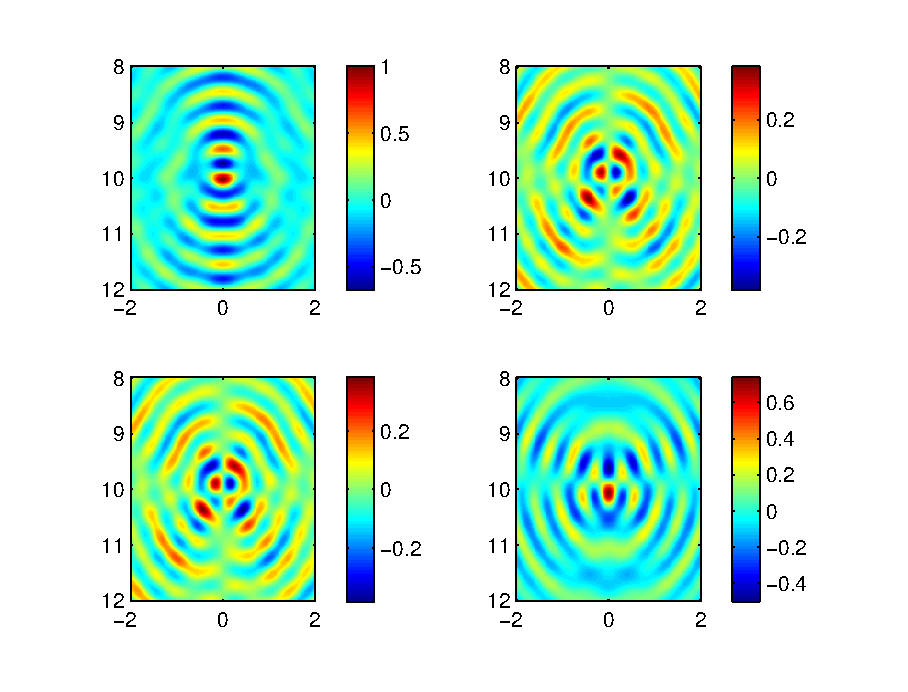
\includegraphics[width=\textwidth]{./Img/graphic/psf_om_2_lm_5_mu_25_im.eps}	
	\caption{$-Im(J_d(z,y))$ for $y=(0,8)^T$, $\omega=2\pi$, $d=100$}\label{figure_green}
\end{figure}
\begin{figure}[htbp]
	\centering
	\includegraphics[width=\textwidth]{./Img/graphic/green_om_2_lm_5_mu_25_im.eps}	
	\caption{$Im(G(z,y))$ for $y=(0,8)^T$, $\omega=2\pi$}\label{figure_psf}
\end{figure}

下面的引理告诉我们,点扩散函数 $\F(z,y)$ 的虚部与弹性波基本解 $\Im\G(z,y)$ 的虚部有相似的函数特性。于是, 利用定理 \ref{J_F_diff} 和引理 \ref{error_jd}, 当 $d\gg h$ 和 $k_s h\gg 1$, 我们可以认为 $\J_d(z,y)$ 的虚部也与弹性波基本解 $\Im\G(z,y)$ 的虚部有相似的函数特性, 见图 \ref{figure_psf} 和 图\ref{figure_green} 所展示。

\begin{remark}
	如图\ref{figure_psf} 和 图\ref{figure_green}中, 每幅图中4副子图, 其中子图的位置对应相应矩阵该位置的函数。其中, 每幅图的采样区域都为 $[-2,2]\times[8,12]$, 角频率 $\om=2\pi$, {Lam\'{e}} 常数 $\lambda=0.5$, $\mu=0.25$。 特别地, 每幅子图中, 颜色越深代表该处的值越大, 因此我们可以看到图\ref{figure_psf} 和 图\ref{figure_green}中对角线上的子图, 他们颜色的最深处正式图的中心位置, 即代表峰值在 $z=y$ 处。
\end{remark}
\begin{thm} \label{thm:3.2}
	对于任意 $z,y\in \R_+^2$, $\F(z,y)^T=\F(z,y)$。 当 $z=y$ 时,  $\Im [\F(z,y)]_{12} = \Im [\F(z,y)]_{21} =0$ 以及
	\be\label{d6}
	-\Im [\F(z,y)]_{ii}\geq \frac{1}{4(\lambda+2\mu)} \ , \ i =1 ,2.
	\ee
	当 $z\neq y$ 时,
	\be\label{d7}
	|\F(z,y)|&\le \frac{C}{\mu}\left(\frac 1{(k_s|z-y|)^{1/2}}+\frac 1{k_s|z-y|}\right),
	\ee
	这里的常数 $C$ 只依赖于 $\kappa$。
\end{thm}

\debproof
将式子 (\ref{d1}) 和式子 (\ref{d2}) 代入式子 (\ref{d4}), 我们可以得到
\be   
\F(z,y)&=&-\frac{1}{2\pi}\int_{-k_p}^{k_p} \frac{\i k_s^2\mu_s}{\mu\gamma(\xi)\delta(\xi)}
\Bigg(
\begin{array}{cc}
	\xi^2 & -\xi\mu_p \\
	-\xi\mu_p & \mu_p^2
\end{array}\Bigg)e^{\i\mu_p (z_2-y_2) +\i\xi(y_1-z_1)}d\xi \nn\\
\hskip-1.5cm& &-\frac{1}{2\pi}\int_{-k_p}^{k_p} \frac{\i k_s^2\mu_p}{\mu\gamma(\xi)\delta(\xi)}
\Bigg(
\begin{array}{cc}
	\mu_s^2 & \xi\mu_s \\
	\xi\mu_s & \xi^2
\end{array}		\Bigg)e^{\i\mu_s (z_2-y_2) +\i\xi(y_1-z_1)}d\xi \nn\\ 
\hskip-1.5cm& &
-\frac{1}{2\pi}\int_{(-k_s,k_s)\bks[-k_p,k_p]} \frac{\i(k_s^2-4\xi^2)\mu_p}{\mu\gamma(\xi)\overline{\delta(\xi)}}
\Bigg(
\begin{array}{cc}
	\mu_s^2 & \xi\mu_s \\
	\xi\mu_s & \xi^2
\end{array}		\Bigg)e^{\i\mu_s (z_2-y_2) +\i\xi(y_1-z_1)}d\xi \nn\\
\hskip-1.5cm&:=&{\rm III}_1+{\rm III}_2+{\rm III}_3. \label{d8}
\ee
由于 $\mu_p(\xi)$ 及 $\mu_s(\xi)$ 关于 $\xi$ 存在对称性, 所以我们易得当 $z=y$ 时, $\Im [\F(z,y)]_{12} = \Im [\F(z,y)]_{21} =0$。

现在我们来证明当 $i=j=1$ 时的不等式(\ref{d6}), 而其他情形时可以被类似证明, 这里将省略细节。 观察到, 当 $\xi\in (-k_p,k_p)$ 时,由引理 \ref{delta} 得 $\delta(\xi)\le k_s^4$ 及易得 $\mu_p\le\mu_s$。 于是当 $z=y$ 时:
\ben
& &-\Im ({\rm III}_1+{\rm III}_2)=\frac{1}{2\pi\mu}\int^{k_p}_{-k_p}\frac{k_s^2\mu_s}{\de(\xi)}d\xi\\
&\geq&\frac{1}{2\pi\mu}\int_{-k_p}^{k_p} \frac{\mu_p}{k_s^2}d\xi = \frac{1}{4(\lambda+2\mu)}.
\een
而当 $\xi\in(-k_s,k_s)\bks[-k_p,k_p]$时,成立 $\mu_p=\i\sqrt{\xi^2-k_p^2}$, 于是我们有
\ben
-{\rm III}_3=\frac{1}{2\pi\mu}\int_{(-k_s,k_s)\bks(-k_p,k_p)} \frac{-\mu_s^2\sqrt{\xi^2-k_p^2}(k_s^2-4\xi^2)}{(\xi^2+\i\mu_s\sqrt{\xi^2-k_p^2})(\varphi^2-\i4\xi^2\mu_s\sqrt{\xi^2-k_p^2})} d\xi.
\een
通过简单的直接计算, 我们有 \ben
\Im[(\xi^2+\i\mu_s\sqrt{\xi^2-k_p^2})(\varphi^2-\i4\xi^2\mu_s\sqrt{\xi^2-k_p^2})]=k_s^2\mu_s\sqrt{\xi^2-k_p^2}(k_s^2-4\xi^2).
\een
 通过分母有理化, 我们可以得到 $-\Im({\rm III}_3)\ge 0$。 因此, 当 $z=y$ 时, 我们有 $-\Im[\F(z,y)]_{11}\ge 1/[4(\lam+2\mu)]$ 。

当 $z\neq y$ 时, 我们可以有如下三角函数表示 $y-z=|y-z|(\cos\phi,\sin\phi)^T$ ,其中 $0\le\phi\le \pi$。 于是, 将此三角变量替换代入 ${\rm III}_1$, 我们可以得到
\ben
{\rm III}_1=\frac{1}{\mu}\int_{0}^{\pi} A(\theta,\kappa) e^{\i k_s |z-y| \cos(\theta-\phi)}d\theta,
\een
显然,简单的代入计算可以得到函数 $A(\theta,\kappa)$ 及其导函数 $\pa A(\theta,\kappa)/\pa\theta$ 在区间 $(0,\pi)$。 而且区间 $(0,\pi)$ 可以分割成若干个互补相交的子区间, 在每个子区间上成立 $|\cos(\theta-\phi)|\ge 1/\sqrt 2$ 或是 $|\sin(\theta-\phi)|\ge 1/\sqrt 2$ 以及 $-\sin(\theta-\phi)$ 在盖子区间上单调。 于是, 当$k_s|z-y|\ge 1$ 时,  Van der Corput 引理 \ref{van} , 我们易得
\ben
|{\rm III}_1|\le \frac C\mu\left(\frac 1{(k_s|z-y|)^{1/2}}+\frac 1{k_s|z-y|}\right).
\een
而当 $k_s|z-y|< 1$ 时,显然有 $|{\rm III}_1|\le C\mu^{-1}\le C\mu^{-1}(k_s|z-y|)^{-1}$。 而针对 ${\rm III}_2+{\rm III}_3$ 的估计可以类似地使用 Van der Corput 引理 \ref{van} 来证明。 引理得证。
\finproof

结合引理 \ref{error_jd}, 定理\ref{J_F_diff}, 定理\ref{thm:3.2} 及图\ref{figure_psf}, 我们发现点扩散函数 $J_d(z,y)$ 确实可以把位于 $y$ 的点源分辨出来, 即在 $z=y$ 处达到峰值, 在 $z$ 远离 $y$ 其值渐渐衰减。


为便于后文分析, 我们介绍如下在范数意义下的估计式。
\begin{lem}\label{lem:4.1}
	令 $k_s h\geq 1, d\gg h$, 存在只依赖于 $\kappa$ 却与 $k_s, h, d, d_D$ 无关的常数 $C$ , 对于任意 $z\in\Om$, $j=1,2$, 成立
	\ben
	& &\|\F(z,\cdot)e_j\|_{H^{1/2}(\Ga_D)}+\|\sigma(\F(z,\cdot)e_j)\nu\|_{H^{-1/2}(\Ga_D)}\le\frac C\mu(1+k_sd_D),\\
	& &\|\R_d(z,\cdot)e_j\|_{H^{1/2}(\Gamma_D)}+\|\sigma(\R_d(z,\cdot)e_j)\nu\|_{H^{-1/2}(\Gamma_D)} \le
	\frac{C}{\mu}(1+k_sd_D)\left[\left(\frac hd\right)^{2}+(k_sh)^{-1/4}\right],
	\een	
	其中 $\R_d(z,\cdot)=\J_d(z,\cdot)-\F(z,\cdot)$.
\end{lem}

\debproof
上面第一估计式可有不等式 (\ref{q0}) 以及 $\F(z,\cdot)$ 的定义 (\ref{d4}) 立即得到。 第二估计式可有不等式 (\ref{q0}), Lemma \ref{error_jd} and Theorem \ref{J_F_diff} 立即得到。这里我们将不再赘述细节。 引理得证。
\finproof

\section{散射系数与 Kirchhoff 逼近}

\subsection{反射面为$x_1$轴}

We consider the scattering of an incident plane $p$-wave  $\hat u_p$ (or $s$-wave $\hat u_s$) with the incident direction $\hat d_0=(\sin t_0, \cos t_0)^T, t_0\in (0,2\pi)$, by the plane $\Gamma := \{x \in \R^2 :x _2 = 0\}$. 
The angle between $\hat d_0$ and the positive real axis is $\theta_0=\pi/2-t_0$. Denote by $\hat\nu=(0,1)^T$.


\subsubsection{$p$-波情形}
We denote the incident $p$-wave \cite[p172]{achenbach1980} as
\ben
\hat u_p=A_0(\sin t_0,\cos t_0)^Te^{\i k_p(x_1\sin t_0+x_2 \cos t_0)}.
\een
The reflected $p$-wave is represented as
\ben
\hat u_{p,p}=A_1(\sin t_1,-\cos t_1)^Te^{\i k_p(x_1\sin t_1-x_2 \cos t_1)}.
\een
The reflected $s$-wave is denoted as
\ben
& &\hat u_{p,s}=A_2(-\cos t_2,-\sin t_2)^Te^{\i k_s(x_1\sin t_2-x_2 \cos t_2)}.
\een
Under the clamped condition, the total field vanishes on $\Ga$ and thus
\ben
\hat u_p(x_1,0)+\hat u_{p,p}(x_1,0)+\hat u_{p,s}(x_1,0)=0,\ \ \forall x_1\in\R.
\een
A simple computation shows that
\ben
t_1=t_0, \ \ \frac{\sin t_2}{\sin t_0}=\frac{k_p}{k_s}:=\kappa, \\
A_0=\cos(t_0-t_2), \ \ A_1=\cos(t_0+t_2), \ \ A_2=\sin 2t_0.
\een
In summary, the total field is
\be\label{a1}
\hat u^{\rm total}_p=A_0\hat d_0e^{\i k_px\cdot\hat d_0}+A_1\hat d_1e^{\i k_px\cdot\hat d_1}+A_2\hat d_2^\perp e^{\i k_s x\cdot\hat d_2},
\ee
where for any $\tau=(\tau_1,\tau_2)^T\in\R^2$, $\tau^\perp=(\tau_2,-\tau_1)^T$, and
\be
\hskip-2cm& &\hat d_1=\hat d_0-2(\hat d_0\cdot\hat\nu)\hat\nu, \hat d_2=\kappa\hat d_0-\left[\kappa(\hat d_0\cdot\hat\nu)+{\rm sgn}(\hat d_0\cdot\hat\nu)\sqrt{1-\kappa^2(\hat d_0\cdot\hat\nu^\perp)^2}\,\right]\hat\nu,\\
\hskip-2cm& &A_0=\hat d_1\cdot\hat d_2, A_1=-\hat d_0\cdot\hat d_2,A_2=2(\hat d_0\cdot\hat\nu)(\hat d_0\cdot\hat\nu^\perp).\label{a2}
\ee

\subsubsection{$s$-波情形}
We denote the incident $s$-wave as 
\ben
& &\hat u_s=A_0(\cos t_0,-\sin t_0)^Te^{\i k_s(x_1\sin t_0+x_2 \cos t_0)}.
\een
The reflected $p$-wave is represented as
\ben
\hat u_{s,p}=A_1(\sin t_1,-\cos t_1)^Te^{\i k_p(x_1\sin t_1-x_2 \cos t_1)}.
\een
The reflected $s$-wave is denoted as
\ben
& &\hat u_{s,s}=A_2(-\cos t_2,-\sin t_2)^Te^{\i k_s(x_1\sin t_2-x_2 \cos t_2)}.
\een
The result is 
\ben
t_2=t_0,\ \ \frac{\sin t_1}{\sin t_0}=\frac{k_s}{k_p}=\kappa_1,\\
A_0=\cos(t_0-t_1),\ \ A_1=-\sin 2t_0,\ \ A_2=\cos(t_0+t_1).
\een
In summary, the total field is
\be\label{b1}
\hat u^{\rm total}_s=A_0\hat d_0^\perp e^{\i k_sx\cdot\hat d_0}+A_1\hat d_1e^{\i k_px\cdot\hat d_1}+A_2\hat d_2^\perp e^{\i k_s x\cdot\hat d_2},
\ee
where 
\be
\hskip-2cm& &\hat d_1=\kappa_1\hat d_0-\left[\kappa_1(\hat d_0\cdot\hat\nu)+{\rm sgn}(\hat d_0\cdot\hat\nu)\sqrt{1-\kappa_1^2(\hat d_0\cdot\hat\nu^\perp)^2}\,\right]\hat\nu, \hat d_2=\hat d_0-2(\hat d_0\cdot\hat\nu)\hat\nu,\\
\hskip-2cm& &A_0=\hat d_1\cdot\hat d_2, A_1=-2(\hat d_0\cdot\hat\nu)(\hat d_0\cdot\hat\nu^\perp),A_2=-\hat d_0\cdot\hat d_1.\label{b2}
\ee

\subsection{反射面为任意平面}

We consider the scattering of an incident plane $p$-wave  $u_p$ or $s$-wave $u_s$ with the incident direction $d=(\sin\theta,\cos\theta)^T,\theta\in (0,2\pi)$, by the plane $\Gamma := \{x \in \R^2 : x \cdot \nu = 0\}$ through the origin with the normal vector $\nu=(\sin\phi,\cos\phi)^T,\phi\in (0,2\pi)$. The angle between $\nu$ and the positive real axis is $\pi/2-\phi$. The total fields are
\be
u_p^{\rm total}=A_0d_0 e^{\i k_p x\cdot d_0}+A_1 d_1 e^{\i k_p x\cdot d_1}+A _2d_2^\perp e^{\i k_s x\cdot d_2},\\
u_s^{\rm total}=A_0d_0^\perp e^{\i k_s x\cdot d_0}+A_1 d_1 e^{\i k_p x\cdot d_1}+A_2 d_2^\perp e^{\i k_s x\cdot d_2},
\ee
where for $i=0,1,2$, $d_i$ is the unit vector and $A_i$ is the corresponding amplitude. We impose $u_p^{\rm total}=0, u_s^{\rm total}=0$ on $\Gamma$. Let  
$\hat x= S x$, where $S\in\R^{2\times 2}$ is the rotation matrix with rotation angle $\phi$,
\ben
S= \left( \begin{array}{ll}
	\cos\phi& -\sin\phi \\
	\sin\phi & \cos\phi
\end{array}\right).
\een
We have $\hat\nu=S\nu$.

\begin{thm}
	Let $u(x)\in \C^2$ and
	\ben
	\Delta_e^x := \left(\begin{array}{ll}
		(\lambda +2\mu)\frac{\pa^2 }{\pa x_1^2}+(\lambda +\mu) \frac{\pa^2}{\pa x_1\pa x_2} +\mu \frac{\pa^2}{\pa x_2^2}\\
		\mu \frac{\pa^2}{\pa x_1^2}+(\lambda +\mu) \frac{\pa^2}{\pa x_1\pa x_2}+(\lambda +2\mu)\frac{\pa^2 }{\pa x_12^2}
	\end{array}\right).
	\een
	Assume that u(x) satisfies $\Delta_e^x u(x)+\omega^2 u(x)=0$, then  we have $\Delta_e^{\hat x} \hat u(\hat x)+\omega^2 \hat u(\hat x)=0$ where $\hat u(\hat x):= S u(S^T\hat x)$ or $u(x)=S^T\hat u(Sx)$.
\end{thm}

\debproof
Since
\ben
\frac{\pa^2}{\pa \hat x_1^2}=\cos^2\phi \frac{\pa^2}{\pa  x_1^2}-2\cos\phi\sin\phi \frac{\pa^2}{\pa  x_1\pa x_2}+\sin^2\phi \frac{\pa^2}{\pa  x_2^2} \\
\frac{\pa^2}{\pa \hat x_2^2}=\sin^2\phi \frac{\pa^2}{\pa  x_1^2}+2\cos\phi\sin\phi \frac{\pa^2}{\pa  x_1\pa x_2}+\cos^2\phi \frac{\pa^2}{\pa  x_2^2} \\
\frac{\pa^2}{\pa \hat x_1 \pa\hat x_2}=\cos\phi\sin\phi\frac{\pa^2}{\pa  x_1^2}+(\cos^2\phi-\sin^2\phi) \frac{\pa^2}{\pa  x_1\pa x_2}-\cos\phi\sin\phi\frac{\pa^2}{\pa  x_2^2}
\een
This completes proof after substituting above equation into $\Delta_e^{\hat x} \hat u(\hat x)$.
\finproof

By this theorem, we obtain from (\ref{a1})-(\ref{a2}) that for $u_p^{\rm total}$, $d_0=(\sin(\theta-\phi),\cos(\theta-\phi))^T$,
\ben
\hskip-2cm& &d_1=d_0-2(d_0\cdot\nu)\nu,d_2=\kappa d_0-\left[\kappa(d_0\cdot\nu)+{\rm sgn}(d_0\cdot\nu)\sqrt{1-\kappa^2(d_0\cdot\nu^\perp)^2}\,\right]\nu, \\
\hskip-2cm& &A_0=d_1\cdot d_2, A_1=-d_0\cdot d_2,A_2=2(d_0\cdot\nu)(d_0\cdot\nu^\perp).
\een
In fact, we have

\ben
u^{\rm total}_p(x)&=&S^T\hat u_p^{\rm total}(Sx)\\
&=&S^T\left[A_0\hat d_0e^{\i k_pSx\cdot\hat d_0}+A_1\hat d_1e^{\i k_pSx\cdot\hat d_1}+A_2\hat d_2^\perp e^{\i k_s Sx\cdot\hat d_2}\right].
\een
This implies $S^T\hat d_j=d_j$, $j=0,1,2$. As $d_0=d$, we obtain $\hat d_0=Sd$.
Similarly, for $u_s^{\rm total}$,  $d_0=(\sin(\theta-\phi),\cos(\theta-\phi))^T$,
\ben
\hskip-2cm& &d_1=\kappa_1 d_0-\left[\kappa_1(d_0\cdot\nu)+{\rm sgn}(d_0\cdot\nu)\sqrt{1-\kappa_1^2(d_0\cdot\nu^\perp)^2}\,\right]\nu, d_2=d_0-2(d_0\cdot\nu)\nu,\\
\hskip-2cm& &A_0=d_1\cdot d_2, A_1=-2(d_0\cdot\nu)(d_0\cdot\nu^\perp),A_2=-d_0\cdot d_1.
\een
The traction of $u(x)$ on the plane $\Gamma$ can be obtained by simple calculation
\be
\sigma(u_p^{\rm total})\cdot\nu&=&[\i k_p A_0 (\lambda\nu+2\mu(d_0,\nu)d_0)+\i k_p A_1 (\lambda\nu+2\mu(d_1,\nu)d_1)\nn\\
& &+\i k_s A_2\mu((d_2,\nu)d_2^\perp+(d_2^\perp,\nu)d_2)]e^{\i k_p x\cdot d_0}\nn\\
&:=&\i k_p A_0 \hat{\mathbf{R}}_p(x,d_0,\nu) e^{\i k_p x\cdot d_0},\label{kir_p}\\
\sigma(u_s^{\rm total})\cdot\nu&=&[\i k_s A_0 \mu((d_0,\nu)d_0^\perp+(d_0^\perp,\nu)d_0)+\i k_p A_1 (\lambda\nu+2\mu(d_1,\nu)d_1)\nn\\
& &+\i k_s A_2\mu((d_2,\nu)d_2^\perp+(d_2^\perp,\nu)d_2)]e^{\i k_s x\cdot d_0}\nn\\
&:=&\i k_s A_0\hat {\mathbf{R}}_s(x,d_0,\nu) e^{\i k_s x\cdot d_0}.\label{kir_s}
\ee


\begin{definition}
	For any unit vector $d\in \R^2$, let $u^i_p =d e^{\i k_p x\cdot d}$ or $u^i_s= d^\perp e^{\i k_s x\cdot d}$ be the incident wave and $u^s_\alpha = u^s_\alpha(x;d)$ be the radiation solution of the Navier equation:
	\ben
	u^s_\alpha + \om^2u^s_\alpha = 0\ \ \mbox{in} \ \  \R^2\bks\bar{D} \\
	\Delta_e	u^s_\alpha =-u^i_\alpha \ \ \mbox{on} \ \ \pa D 
	\een
	The scattering coefficient $\mathbf{R}_\alpha(x;d)$ for $x\in\pa D$ is defined by the relation
	\ben
	\sigma(u^s_\alpha+u^i_\alpha)\cdot \nu= \i k_\alpha \mathbf{R}_\alpha(x;d)e^{\i k_\alpha x\cdot d}  \ \ \ \mbox{on}\ \ \pa D
	\een
	where $\alpha=p,s$.
\end{definition}

For a convex object $D$, Kirchhoff approximation approximates the scattering coefficient by considering 
the boundary at $x\in\pa D$ locally as a plane with normal $\nu$ to obtain
\ben
\mathbf{R}_\alpha(x;d)\approx\left\{ \begin{array}{ll}
	\hat {\mathbf{R}}_\alpha(x;d,\nu(x))    \ \  \  \mbox{if} \ \ x \in \pa D^{-}_d=\{x\in \pa D, \nu(x)\cdot d<0\},\\ 
	0 \ \ \ \ \ \ \ \  \ \ \ \ \ \ \ \ \mbox{if} \ \ x \in \pa D^{+}_d=\{x\in \pa D, \nu(x)\cdot d\geq0\}.
\end{array} \right.
\een


\subsection{数值算例}
In this section we present several numerical examples to show the effectiveness of Kirchhoff approximation. To synthesize the real scattering coefficient we compute the solution $\sigma(u^s_\alpha+u^i_\alpha)\cdot \nu$ of
the scattering problems by representing the ansatz solution as the single layer potential
with the Green tensor $\G(x,y)$ as the kernel
\ben\hspace{-2cm}
u^s(x)=\int_{\Ga_D} - \G(y,x)^T\sigma(u^s(y)+u^i(y))\nu ds(y)=-u^i(x) \ \ \ \  \mbox{on} \ \ x\in \Ga_D,
\een 
and discretizing the integral equation by
standard Nystr\"{o}m methods \cite{colton-kress}. Let $\mathbf{R}_\alpha(x;d)=(\mathbf{R}_\alpha^1(x;d),\mathbf{R}_\alpha^2(x;d))^T$, then we have
\be
\mathbf{R}_\alpha^j(x;d)=\frac{\sigma(u^s(y)+u^i(y))\nu\cdot e_j}{\i k_\alpha e^{\i k_\alpha x\cdot d} }.
\ee
We compute $\hat {\mathbf{R}}_\alpha(x;d)=(\hat {\mathbf{R}}_\alpha^1(x;d),\hat {\mathbf{R}}_\alpha^2(x;d))^T$ by (\ref{kir_p}) and (\ref{kir_s}).
In all our numerical examples we choose {Lam\'{e}} constant $\lambda=1/2$, $\mu=1/4$ and 
\ben
u^i_p=(\cos t,\sin t )^T e^{\i k_p(x_1 \cos t +x_2\sin t)} \\
u^i_s=(\sin t,-\cos t)^T e^{\i k_s(x_1 \cos t +x_2\sin t)}
\een where
$t\in[0,2\pi]$.. 
The boundaries
of the obstacles used in our numerical experiments are parameterized as follows:
\ben
\hskip-2cm\mbox{Circle:}\ \ \ \ x_1=\cos(\theta),\ \ x_2=\sin(\theta);\ \  \\
\hskip-2cm\mbox{Pear:}\ \ \ \rho = 0.5(2+0.3\cos(3\theta)),x_1=\sin \frac{\pi}{4}\rho(\cos\theta-\sin\theta),x_2=\sin \frac{\pi}{4}\rho(\cos\theta+\sin\theta),
\een
where

$\theta\in[0,2\pi]$ (See Figure \ref{shape}). 

In the following examples, we take the angular frequency $\omega= \pi,2\pi,4\pi,8\pi$.

\begin{figure}[htbp]
	\centering
	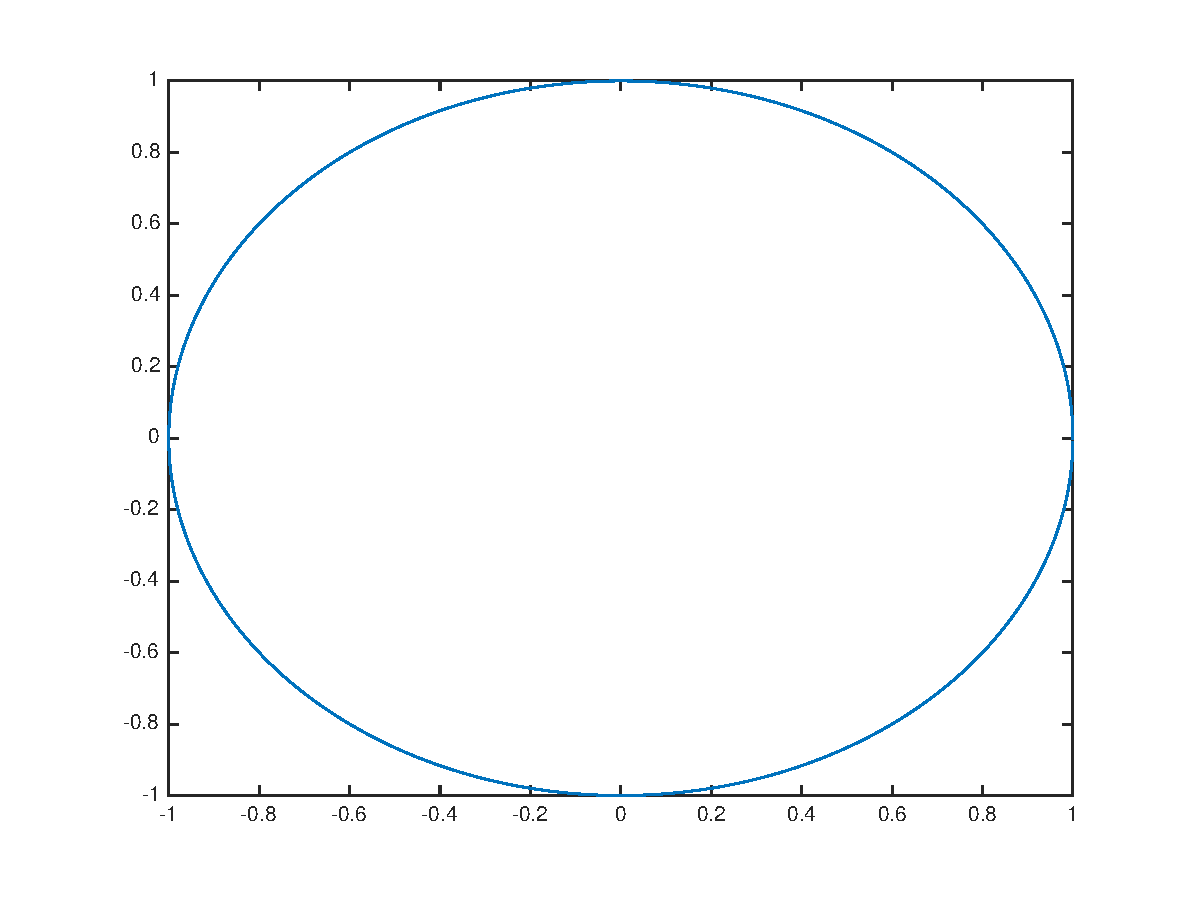
\includegraphics[width=0.48\textwidth]{./Img/figure_sc_elastic/circle.eps}
	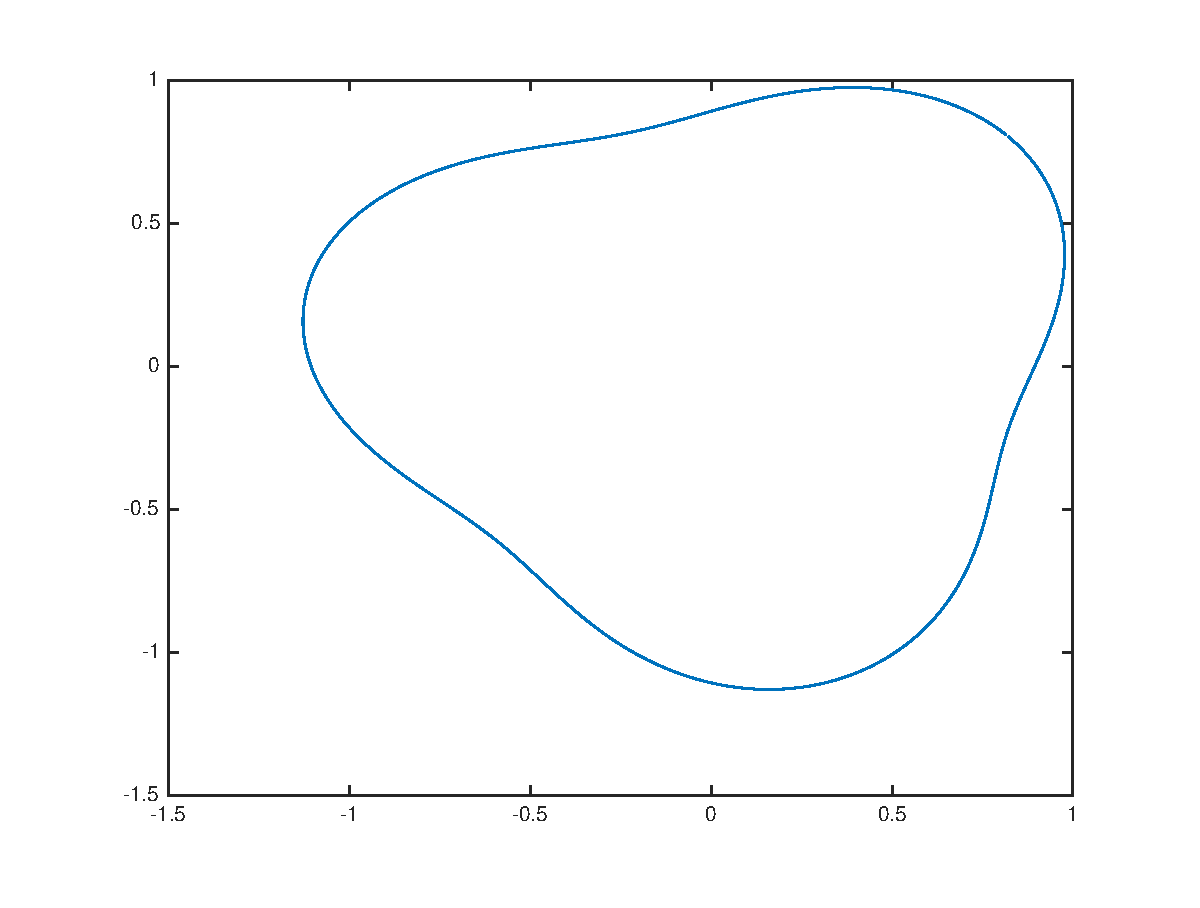
\includegraphics[width=0.48\textwidth]{./Img/figure_sc_elastic/pear.eps}
	\caption{The shape of the obstacles.}\label{shape}
\end{figure}




